\documentclass[UTF8]{ctexart}
\hfuzz=4pt

\usepackage{parskip}
    \setlength{\parindent}{0em}
\usepackage{geometry}
    \geometry{left=4cm,right=4cm,top=2cm,bottom=2cm}
\usepackage{amsmath, amssymb, amsthm, mathtools}
\usepackage{thmtools}
    \renewcommand\qedsymbol{$\blacksquare$}
    \declaretheorem[numberwithin=section,shaded={rulecolor=cyan,rulewidth=2pt,bgcolor=white}]{definition}
    \declaretheorem[numberwithin=section,shaded={rulecolor=orange,rulewidth=2pt, bgcolor=white}]{theorem} 
    \newtheoremstyle{mystyle}{1em plus .2 em minus .2em}{1em plus .2 em minus .2em}{}{}{\bfseries}{.}{.5em}{}
    \theoremstyle{mystyle}
    \newtheorem{axiom}{Axiom}[section]
    \newtheorem{lemma}{Lemma}[section]
    \newtheorem{proposition}{Proposition}[section]
    \newtheoremstyle{myremark}{1em plus .2 em minus .2em}{1em plus .2 em minus .2em}{}{}{\itshape}{.}{.5em}{}
    \theoremstyle{myremark}
    \newtheorem*{remark}{Remark}
    \theoremstyle{plain}
    \newtheorem{corollary}{Corollary}[section]
\usepackage{caption}
\usepackage{xcolor}
\usepackage{graphicx}
\usepackage{float}
\usepackage{setspace} 	 % 行间距 \begin{spacing}{arg}
\usepackage{esint}
\usepackage{hyperref}
    \hypersetup{colorlinks=true,linktoc=all,linkcolor=blue}

\newcommand{\ve}[1]{\boldsymbol{\mathbf{#1}}}
\newcommand{\unit}[1]{\boldsymbol{\mathbf{\hat{#1}}}}
\renewcommand{\r}{\mathrm}
\renewcommand{\cal}{\mathcal}
\newcommand{\scr}{\mathscr}

\newcommand{\E}{\mathrm e}
\renewcommand{\I}{\mathrm i}
\newcommand{\R}{\mathbb R}
\newcommand{\Z}{\mathbb Z}
\newcommand{\N}{\mathbb N}
\newcommand{\Q}{\mathbb Q}
\renewcommand{\C}{\mathbb C}
\DeclarePairedDelimiter\set{\{}{\}}
\def \DD #1.#2.#3 {\dfrac{d^{#1} #2}{d #3^{#1}}}
\def \PP #1.#2.#3 {\dfrac{\partial^{#1} #2}{\partial #3^{#1}}}
\def \dd #1.#2 {\dfrac{d #1}{d #2}}
\def \pp #1.#2 {\dfrac{\partial #1}{\partial #2}} 
\newcommand{\del}{\nabla}


\pagestyle{empty}

\begin{document}
\section{二元关系}
\subsection{关系的定义}
集合 $ A $ 到 $ B $ 的一个二元关系 $ R $ 是 $ A \times B $ 的子集.

\paragraph{例}
$ A = \set{a, b} $, $ B = \set{1, 2} $. 则 $ A \times B = \set{(a, 1), (a, 2), (b, 1), (b, 2)} $. 任取 $ A \times B $ 的一个子集, 就是 $ A $ 到 $ B $ 的一种关系: 如 $ R = \set{(a, 1), (b, 1)} $.

\begin{definition}[\text{关系的复合}]
    设集合 $ A $ 到 $ B $ 的关系 $ R $, 以及 $ B $ 到 $ C $ 的关系 $ S $. 则 $ R $ 与 $ S $ 的复合 $ R \circ S $ 定义为:
    \[ R \circ S \coloneqq \set{(a, c) \mid \exists b \in B \text{ 使得 } (a, b) \in R \land (b, c) \in S} \,.\]
\end{definition}

\begin{proposition}[\text{复合的性质}] \ 
    \begin{itemize}
        \item (结合律) $ (R \circ S) \circ T = R \circ (S \circ T) $
        \item (恒等关系) $ R \circ I_A = R $, $ I_A \circ R = R $
        \item (逆关系) $ R^{-1} \circ R = I_A $, $ R \circ R^{-1} = I_A $
        \item $ (R \circ S)^{-1} = S^{-1} \circ R^{-1} $
    \end{itemize}
\end{proposition}


递归地定义 $ R^n $:
\[ R^n \coloneqq \begin{cases}
    I_A & n = 0 \\
    R^{n - 1} \circ R & n > 0
\end{cases} \,.\]

于是有:
\[ \begin{array}{c}
    R^0 = I_A \\
    R^1 = I_A \circ R = R \\
    R^2 = R^1 \circ R = R \circ R \\
    R^3 = R^2 \circ R = R \circ R \circ R
\end{array} \]

\begin{theorem}[\text{传递性}]
    集合 $ A $ 上的关系 $ R $ 具有传递性, 当且仅当 $ R^n \subseteq R $ 对 $ n \in \Z^+ $ 成立.
\end{theorem}

\begin{proof} \ \\
    正推: $ R^n \subseteq R $ 在 $ n = 1 $ 时成立, 此为基础情形. 现归纳地假设对于 $ n \geqslant 1 $, $ R^n \subseteq R $. 要证明 $ R^{n + 1} \subseteq R $. 对于 $ (a, b) \in R^{n + 1} $, 存在 $ c \in A $, $ (a, c) \in R^n $, $ (c, b) \in R $. 根据归纳假设, $ (a, c) $ 也一定在 $ R $ 中. 于是 $ (a, c) \in R $ 且 $ (c, b) \in R $, 由于传递性, $ (a, b) \in R $, 所以 $ R^{n + 1} \subseteq R $.
    
    反推: 设 $ R^n \subseteq R $ 对任意整数 $ n \geqslant 1 $ 成立. 若 $ (a, b) \in R $ 且 $ (b, c) \in R $, 则有 $ (a, c) \in R^2 $, 而 $ R^2 \subseteq R $, 所以 $ (a, c) \in R $. 这说明了传递性.
\end{proof}





\section{序集}
\subsection{偏序}
\begin{definition}[\text{偏序集}]
    集合 $ X $ 连同其上的关系 $ \le $ 一起 $ (X, \le) $ 被称为偏序集 (partially ordered set, poset), 当且仅当其满足以下三条性质:
    \begin{itemize}
        \item 自反 (reflexive): $ \forall x \in X $, $ x \le x $
        \item 反对称 (anti-symmetric): $ \forall x, y \in X $, $ x \le y $ 且 $ y \le x $ 则 $ x = y $
        \item 传递 (transitive): $ \forall x, y, z \in X $, $ x \le y $ 且 $ y \le z $ 则 $ x \le z $
    \end{itemize}
\end{definition}

严格地说, $ (X, \le) $ 才是偏序集, 但当 $ \le $ 已知的时候, 常常省略关系 $ \le $, 称 $ X $ 是一个偏序集. 另外, 为了描述关系所述的集合, 可以使用 $ \le_X $ 表示 $ \le $ 是 $ X $ 上的关系. 同理, 若确信不会带来混乱, 我们也常常省略下标.


\begin{definition}[\text{严格偏序}]
    在偏序集 $ X $ 上使用记号 $ x < y $ 表示 $ x \le y $ 且 $ x \neq y $, 称关系 $ < $ 为严格偏序. 于是, 严格偏序 $ (X, <) $ 满足:
    \begin{itemize}
        \item 非自反 (irreflexive): $ \forall x \in X $, $ x \not < x $
        \item 非对称 (assymmetric): $ \forall x, y \in X $, $ x < y $, 则 $ y \not < x $
        \item 传递 (transitive): $ \forall x, y, z \in X $, $ x < y $ 且 $ y < z $ 则 $ x < z $
    \end{itemize}
\end{definition}

\begin{remark}
    一旦定义了偏序 $ \le $, 则对应的记号 $ \ge $ 就随之定义: $ x \ge y $ 被定义为 $ y \le x $. 严格偏序同理, $ x < y $ 等价于 $ y > x $. 此外, 注意 $ x \le y $ 等价于 $ x < y $ 或 $ x = y $.
\end{remark}

应当注意一点, 偏序集 $ (X, \le) $ 中, 任意两个元素 $ x $, $ y $ 一定处于且仅处于下面四种情况中的一种:
\begin{itemize}
    \item $ x > y $
    \item $ x = y $
    \item $ x < y $
    \item $ x $, $ y $ 不可比较 (incomparable)
\end{itemize}

若 $ x $, $ y $ 满足其中前三种情况的一种 $ x < y $ 或 $ x = y $ 或 $ x > y $, 则称 $ x $ 和 $ y $ 是可比较的 (comparable).

\subsection{全序}
\begin{definition}[\text{全序集}]
    若偏序集 $ X $ 中任意两个元素 $ x $, $ y $ 都是可比较的, 则称 $ X $ 是一个全序集 (totally ordered set, toset) 或链 (chain).
\end{definition}

\begin{remark}
    称全序集为链, 是因为在 Hasse 图中, 所有元素从上到下排成了一条链, 因为任意两个元素都是可以``比较大小''的.
\end{remark}

也就是说, 全序集是特殊的偏序集, 是偏序集的加强版本.

\subsection{序集上的性质}
首先是序集及其子集的性质.

\begin{proposition}
    偏序集的子集仍然是偏序集, 全序集的子集仍然是全序集.
\end{proposition}

由于 $ X $ 是偏序集, $ Y $ 是 $ X $ 的子集, $ Y $ 中的元素都在 $ X $ 中, 可以看出 $ X $ 中元素满足的自反、反对称、传递性, $ Y $ 中的元素也应该满足. 全序集及其子集同理. 具体证明过程省略.

\subsubsection{最大元与极大元}
下面就来研究偏序集的子集上的一些特别元素及其性质.

\begin{definition}[\text{极大元 (Maximal element)}]
    $ X $ 是偏序集, $ Y $ 是 $ X $ 的子集. 若 $ m \in Y $, 则 $ m $ 是 $ Y $ 的极大元, 当且仅当不存在 $ y \in Y $, $ y > m $. 换句话说, $ Y $ 中没有比 $ m $ 更大的元素. 
\end{definition}

\begin{remark}
    不存在 $ y \in Y $, $ y > m $ 的等价表述为: 对于所有 $ y \in Y $, 要么 $ y \le m $, 要么 $ y $ 和 $ m $ 不可比. 因为 $ x $ 和 $ y $ 只有四种状态 (见前文).
\end{remark}

\begin{definition}[\text{最大元 (Greatest element)}]
    $ X $ 是偏序集, $ Y \subseteq X $. 若 $ m \in Y $, 则 $ m $ 是 $ Y $ 的极大元, 当且仅当 $ \forall y \in Y $, $ m \ge y $. 换句话说, $ m $ 大于 $ Y $ 中所有元素.
\end{definition}

极小元 (minimal element) 和最小元 (least element) 可以同理定义.

\begin{remark}
    由定义可以看出, 最大元蕴含极大元, 所以最大元比极大元更强. 最大元一定是极大元, 但极大元不一定是最大元.
\end{remark}


极大元和最大元是不同的概念. $ Y $ 中没有比 $ m $ 更大的元素, 不能说明 $ m $ 大于 $ Y $ 中所有元素. 考虑下面的偏序集 $ Y = \set{\varnothing, \set{1}, \set{1, 2}, \set{1, 3}} $ 及其上的偏序 $ \subseteq $: $ \set{1, 2} $ 是极大元, 没有比 $ \set{1, 2} $ 更大的元素, 因为在 $ Y $ 中找不到 $ y $ 满足 $ \set{1, 2} \subseteq y $. 同理 $ \set{1, 3} $ 也是极大元. 由此看出极大/小元可以不唯一.

在 Hasse 图上, 极大元和极小元就是图的顶和底, 但可以不唯一. 

\begin{figure}[H]
    \centering
    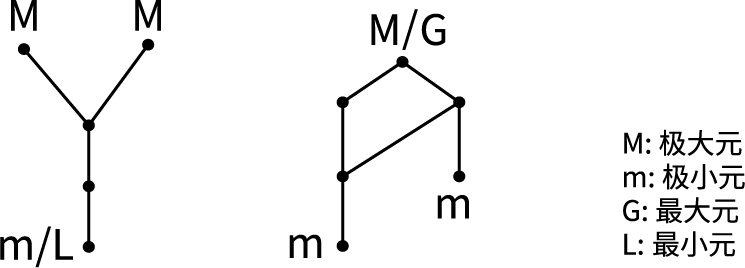
\includegraphics[width = 0.6\linewidth]{./images/maximal_greatest.png}
\end{figure} 

考虑 $ X = (0, 1) \subseteq \R $ 和小于等于关系 $ \leqslant $, $ X $ 没有极大元和最大元. 考虑 $ X = \set{\set{1}, \set{2}, \set{1, 2}} $ 和子集关系 $ \subseteq $, $ X $ 有唯一极大元 $ \set{1, 2} $ 和唯一最大元 $ \set{1, 2} $. 设集合:
\[ A = \set{\set{n} \colon n, k \in \N, n \leqslant k} \,,\]

直观地说, $ A = \set{\set{0}, \set{1}, \set{2}, \dots, \set{k}} $.

那么考虑集合 $ A \cup \set{\varnothing} = \set{\varnothing, \set{0}, \set{1}, \dots, \set{k}} $. 这个偏序集 $ (A, \subseteq) $ 有 $ k $ 个极大元, $ 0 $ 个最大元.

由此看出:

\begin{proposition}
    $ X $ 为偏序集, 则 $ X $ 可能没有极大元, 或有任意个极大元. $ X $ 可能没有最大元或存在唯一最大元. 极小元和最小元同理.
\end{proposition}

\begin{proposition}
    $ X $ 为偏序集, 若存在最大元, 则最大元是唯一的. 且此时极大元也是唯一的, 等于最大元. 也就是说, 最大元存在时, 极大元和最大元等价. 极小元和最小元同理.
\end{proposition}

\begin{remark}
    注意上面的逆命题并不成立, 若 $ X $ 有唯一极大元 $ x $, 则 $ x $ 不一定是 $ X $ 的最大元. (如果限制到有限的偏序集上, 情况如何?)

    针对这个逆命题, 我们可以举出反例, 定义集合 $ S_k \coloneqq \set{n \in \Z \colon 0 \leqslant n \leqslant k} $. 也就是说, $ S_k $ 为 $ 0 $ 到 $ k $ 的整数组成的集合:
    \[ \begin{array}{c}
        S_0 = \set{0} \\
        S_1 = \set{0, 1} \\
        S_2 = \set{0, 1, 2} \\
        S_n = \set{0, 1, 2, \dots, n}
    \end{array} \,.\]

    考虑集合 $ A = \set{S_n \colon n \in \N} \cup \set{\set{0, -1}} $, 即:
    \[ A = \set{\set{0, -1}, \set{0}, \set{0, 1}, \set{0, 1, 2}, \dots} \,.\]

    这是一个无限集, 其有唯一极大元 $ \set{0, -1} $, 但没有最大元.
\end{remark}

\begin{proof}
    设 $ (X, \le) $ 的一个子集 $ Y $ 存在最大元 $ m $. 假设存在另一个最大元 $ m' $, 按照定义 $ m, m' \in Y $, 且应该有 $ m \ge m' $ 和 $ m' \ge m $, 所以 $ m' = m $. 这说明最大元如果存在, 必然是唯一的.

    假设存在极大元 $ n $, $ n \in Y $, 所以有 $ m \ge n $.
    由于 $ m \in Y $, 所以要么 $ n \ge m $, 要么 $ n $ 和 $ m $ 不可比. 由于已经有 $ m \ge n $, 说明两者是可比的. 所以只可能 $ n \ge m $, 又有 $ m \ge n $, 则 $ m = n $. 这说明最大元存在时, 极大元是唯一等于最大元的.
\end{proof}

\begin{corollary} (?)
    若 $ X $ 是一个有限的偏序集, 且 $ X $ 存在唯一极大元 $ x $, 则 $ x $ 就是 $ X $ 的最大元.
\end{corollary}

\begin{proof}
    设 $ X $ 是一个有限的 $ n $ 元偏序集, 其有唯一极大元 $ x $. 按照定义, $ \forall y \in X $, 要么 $ y \le x $, 要么两者不可比. 于是可以分出两种情况: (1) 对任意 $ y \in X $, 都有 $ y \le x $; (2) 存在 $ y \in X $, $ x $ 不可比.

    (1) 若所有 $ y \in X $ 都有 $ y \le x $: 按照定义, $ x $ 为最大元.

    (2) 若 $ X $ 中存在与 $ x $ 不可比的元素: 记作 $ y_1 $. 下面归纳地假设 $ X $ 中存在与 $ x $ 不可比的 $ y_i $. 要证明 $ X $ 中一定存在与 $ x $ 不可比的 $ y_{i + 1} > y_i $.

    首先一定存在 $ y_{i + 1} \in X $, $ y_{i + 1} > y_i $. 因为如果不存在此元素, 按照定义 $ y_i $ 成为极大元. 而 $ y_i $ 与 $ x $ 不可比, $ y_i \neq x $. 于是 $ X $ 有两个不同的极大元, 不符合题述唯一极大元的条件.

    其次 $ y_{i + 1} $ 和 $ x $ 一定是不可比的. 因为一旦可比, $ x \le y_{i + 1} $ 会导致 $ x $ 不是极大元; 而 $ y_{i + 1} \le x $ 会导致 $ y_i < y_{i + 1} \le x $ 即 $ y_i $ 和 $ x $ 可比.

    所以完成了归纳. 这意味着只要存在一个和 $ x $ 不可比的 $ y_1 \in X $, $ X $ 中就会存在无穷个元素 $ y_1, y_2, \dots $, 每个都是与 $ x $ 不可比的, 且这些元素互不相同: $ y_1 < y_2 < \cdots $. 但 $ X $ 是有限集, 这就产生了矛盾. 
    
    所以情况 (2) 是不存在的, 只有情况 (1) 成立, 此时 $ x $ 为最大元.
\end{proof}

\begin{proposition}
    $ X $ 为全序集, 则最大元和极大元始终等价. 极小元和最小元同理.
\end{proposition}

\begin{proof} 
    证明两部分: 最大元蕴含极大元; 极大元蕴含最大元.


    
\end{proof}

总结一下, 偏序集中: 极大元和最大元是两个不同的概念. 极大元可以有零个或任意个, 最大元只能有零个或一个. 且当最大元存在时, 两者等价, 此时两者都是唯一的.

而全序集中, 由于可比性: 最大元和极大元是始终等价的概念, 要么同时没有, 要么同时有唯一相同的最大元和极大元.

\paragraph{最大元和极大元的个数情况} \ 

偏序集中, 最大元和极大元有四种情况:
\begin{itemize}
    \item $ 0 $ 个极大元, $ 0 $ 个最大元
    \item $ 1 $ 个极大元, $ 0 $ 个最大元 (若偏序集有限, 不可能出现这种情况 ?)
    \item $ 1 $ 个极大元, $ 1 $ 个最大元
    \item 多个极大元, $ 0 $ 个最大元
\end{itemize}

全序集中, 最大元和极大元等价, 有两种情况:
\begin{itemize}
    \item $ 0 $ 个极大元, $ 0 $ 个最大元
    \item $ 1 $ 个极大元, $ 1 $ 个最大元
\end{itemize}


\subsubsection{上界与最小上界}
\begin{definition}[\text{上界 (upper bound)}]
    设 $ Y $ 是偏序集 $ X $ 的子集. 对于 $ \beta \in X $, 称 $ \beta $ 为 $ Y $ 的上界, 当且仅当 $ \forall y \in Y $, $ \beta \ge y $.
\end{definition}

\begin{definition}[\text{最小上界}]
    设 $ Y $ 是偏序集 $ X $ 的子集. 设 $ \beta \in X $ 为 $ Y $ 的上界, 称 $ \beta $ 为 $ Y $ 的最小上界, 当且仅当对于任意 $ Y $ 的上界 $ \beta' $ 满足 $ \beta \le \beta' $. 即 $ \beta $ 是所有上界的集合的最小元.
\end{definition}

同理可以定义下界 (lower bound) 和最大下界 (greatest lower bound).

\begin{remark}
    $ Y $ 的极大/小元和最大/小元都是 $ Y $ 中的元素, 而 $ Y $ 的上/下界和最小上界/最大下界却可以是 $ Y $ 外的元素.
\end{remark}

\begin{proposition}
    一个偏序集可以没有上界, 或存在任意个上界; 可以没有最小下界, 或存在唯一最小下界. 下界和最大下界同理.
\end{proposition}

\begin{proposition}
    设 $ Y $ 是偏序集 $ X $ 的子集. 若 $ \beta $ 为 $ Y $ 的一个上界, 若 $ \beta \in Y $, 则有下面两条结论:
    \begin{itemize}
        \item $ \beta $ 为 $ Y $ 的最小上界
        \item $ \beta $ 为 $ Y $ 的最大元
    \end{itemize}

    这就导出了最大元的等价定义: 若 $ Y $ 中存在元素等于最小上界, 则这个元素为最大元. 下界和最大下界同理.
\end{proposition}


\end{document}